\chapter{Trust: Audit, Failure and the Road Ahead}\label{ch10}
\InputIfFileExists{figures/ch10_numbers}{}{}
\directlua{
  function ch10_brkident(s)
    local bs = string.char(92)
    s = string.gsub(s, bs .. "_", "_")
    local prev = ""
    for _, c in utf8.codes(s) do
      local ch = utf8.char(c)
      if string.find(prev, "^[a-z]$") and string.find(ch, "^[A-Z]$") then tex.sprint(bs .. "allowbreak{}") end
      tex.sprint(-2, ch)
      if ch == "/" or ch == "_" or ch == "." then tex.sprint(bs .. "allowbreak{}") end
      prev = ch
    end
  end
}
\newcommand{\brkident}[1]{\texttt{\directlua{ch10_brkident("\luaescapestring{\detokenize{#1}}")}}}% identifier or path in running text, breakable after / . _ and before a capital

On 9~October 2026, when the estimators that turn tracked vortex positions into a friction coefficient had just been ported to a second language, the
programme's own known-answer test --- which the original implementation had passed, once --- was run on \NxGateSeeds{} seeds instead of one. The test is simple. \NxGateTracks{} synthetic tracks of up to \NxGateTend{} time units (a track stops when a vortex and an antivortex come within a distance $2$, the box having side $64$) are generated from a model in which the friction
of a vortex, $\alpha=\NxGateAlpha$, has been put in by hand; the estimator receives the tracks and must give $\alpha$ back. When the model vortices
do not diffuse, the \emph{energy estimator} returns \NxGateEnergyZ. When they diffuse, with $\eta=5\times10^{-4}$, $10^{-3}$ and $2\times10^{-3}$, it
returns \NxGateEnergyA, \NxGateEnergyB and \NxGateEnergyC: too low by \NxGateBiaseA, \NxGateBiaseB and \NxGateBiaseC~percent. On the one seed with
which the test had first been run it had returned \NxQGateSeedEnergy, inside the registered tolerance of 15~percent, and the gate had been recorded
as passed.

The estimator was not wrong in a way that a proof could have caught. The identity on which it rests is a theorem of the library
(\Lthm{DissipativeVortexDynamics}{energy_dissipation}, section~\ref{ch10:sec-estimator}), and the theorem is true. It had been applied to data that
do not satisfy its hypothesis, and no instrument the programme owned at that moment could say so: not the proof assistant, which had never been
asked about the data; not the original implementation, which computed the same quantity in the same way; and not the gate, which had been run once.

That is the subject of this last chapter. The book has used three instruments together --- an experiment, a proof assistant, a solver --- and each
of them vouches for something different and for nothing else. Here we ask what that something is, what it is not, and what happened in the
programme behind the book when an instrument was trusted past its warranty. The chapter works the estimator example through, with the proved
statement, the solver run and the comparison between them (section~\ref{ch10:sec-estimator}); lays out what each kind of check can and cannot see
(section~\ref{ch10:sec-checks}); reports the audit of the Lean library carried out for this book, including what it corrected in the programme's own
records (section~\ref{ch10:sec-audit}); tells the failures of the programme from its ledger (section~\ref{ch10:sec-failures}) and the status of its
speed claims (section~\ref{ch10:sec-speed}); and closes with what a reader can reuse and what is still open
(sections~\ref{ch10:sec-legacy} and~\ref{ch10:sec-open}).

%=====================================================================================================================================
\section{A number that passed once}\label{ch10:sec-estimator}

\subsection*{The model and the two estimators}

\Cref{ch07} develops the motion of a quantized vortex in a thermal bath; we need only its bookkeeping. In the point-vortex description a vortex of
charge $q_i=\pm1$ at position $\mathbf r_i$ in a periodic box moves as
\begin{equation}\label{ch10:eq-model}
  \dot{\mathbf r}_i=(1-\alpha')\,\mathbf v_{s,i}-\alpha\,q_i\,\hat z\times\mathbf v_{s,i}+\sqrt{2\eta}\,\boldsymbol\xi_i(t),
\end{equation}
in units $\hbar=m=1$ (circulation $2\pi$). Here $\mathbf v_{s,i}$ is the velocity that the other vortices induce at $\mathbf r_i$, $\alpha$ is the
longitudinal friction, $\alpha'$ its transverse partner, $\eta$ the diffusion constant of one vortex and $\boldsymbol\xi_i$ unit white noise. Without
the noise term this is a gradient flow with a skew part. With $H$ the vortex energy ($H=-\sum_{i<j}q_iq_j\ln r_{ij}^2$ in the plane, the
Weiss--McWilliams sum on the torus) it reads $\dot{\mathbf r}=A(\nabla H)-\tfrac{\alpha}{2}\nabla H$, where $A$ is skew at every point and carries
$\alpha'$.

Two estimators of $\alpha$ are applied to tracked positions. The \emph{energy estimator} uses the fact that, without noise, $H$ changes only through
the friction: $\alpha=-\dot H/\bigl(2\sum_i|\mathbf v_{s,i}|^2\bigr)$. On a track it is minus the slope of $H(t)$ against the running integral
$\int 2\sum_i|\mathbf v_{s,i}|^2\,\mathrm dt$. The \emph{regression estimator} regresses the displacement of every vortex over a fixed lag on two
predictors, $\int\mathbf v_s\,\mathrm dt$ and $\int(-q\,\hat z\times\mathbf v_s)\,\mathrm dt$; the two coefficients are $1-\alpha'$ and $\alpha$, and
the scatter of the residual gives $\eta$. The first needs only the energy of the configuration; the second needs the positions, and is the one that
also delivers $\alpha'$ and $\eta$.

\subsection*{What Lean proves about the energy estimator}

\begin{leanbox}{DissipativeVortexDynamics}
\begin{lstlisting}[style=lean]
/-- `r' = A(∇H) − γ ∇H` with `A` pointwise skew gives `d/dt H(r) = −γ ‖∇H‖²`. -/
theorem energy_dissipation (H : X → ℝ) (gradH : X → X) (hH : ∀ x, HasGradientAt H (gradH x) x)
    (A : X → X) (hA : ∀ v, inner ℝ v (A v) = 0) (γ : ℝ) (r : ℝ → X)
    (hr : ∀ t, HasDerivAt r (A (gradH (r t)) - γ • gradH (r t)) t) (t : ℝ) :
    HasDerivAt (fun t => H (r t)) (-γ * ‖gradH (r t)‖ ^ 2) t := by
  have h := (hH (r t)).hasFDerivAt.comp_hasDerivAt t (hr t)
  have e : (InnerProductSpace.toDual ℝ X (gradH (r t))) (A (gradH (r t)) - γ • gradH (r t))
      = -γ * ‖gradH (r t)‖ ^ 2 := by
    rw [InnerProductSpace.toDual_apply_apply, inner_sub_right, hA, inner_smul_right,
      real_inner_self_eq_norm_sq]; ring
  rw [e] at h
  exact h
\end{lstlisting}
\end{leanbox}

Read the statement as follows. The space $X$ is a real inner-product space (here the configuration space of all the vortices); $H$ has a gradient
at every point; $A$ is skew, $\langle v,Av\rangle=0$; and the path $r(t)$ solves $\dot r=A\nabla H-\gamma\nabla H$ at \emph{every} time. Then
$H(r(t))$ is differentiable and its derivative is $-\gamma\|\nabla H(r(t))\|^2$, whatever the skew part. The proof is the chain rule, the skew
symmetry of $A$ and $\langle v,v\rangle=\|v\|^2$; it is the eight lines above, shown whole. Two companions complete it:
\Lthm{DissipativeVortexDynamics}{dissipation_indep_of_skew} says that the dissipation rate at a configuration does not depend on the skew part (so
the energy estimator knows nothing about $\alpha'$), and \Lthm{DissipativeVortexDynamics}{energy_antitone} says that for $\gamma\ge0$ the vortex
energy never increases.

The docstring of the module is exact about the scope of what has been formalised: ``What is formal is that the estimators used on the data are
identities of the model.'' That sentence is the point of this section. The identity is a fact about solutions of the model; whether a track
extracted from a simulated field is such a solution is a different question, which must be put to the data. The hypothesis \texttt{hr} demands a
derivative at every time. A vortex with $\eta>0$ has none: its path is a diffusion. The theorem does not apply to a thermal field, and nothing in the
proof assistant objects when a script applies the estimator to one.

\subsection*{What the solver shows}

To find out what the estimator does when the hypothesis fails one needs a case in which the truth is known. That is the registered synthetic gate G0
(\cref{ch07} gives its role in the campaign): tracks are generated from the model (\ref{ch10:eq-model}) with $\alpha=\NxGateAlpha$,
$\alpha'=\NxGateAlphap$, $\eta=\NxGateEta$ and detection noise added to the positions, and the estimators must return the numbers that were put in.
We ran it with the rusty-SUNDIALS example \texttt{g0\_scan}, a Rust program that contains both the Langevin generator and the estimators of the
\texttt{qf-pgpe} crate, on seeds $0,\dots,7$ (the seeds are deterministic, so the run can be repeated exactly).

\begin{rustbox}{the registered synthetic gate G0, many seeds}
\begin{lstlisting}[style=plainmono]
$ g0_scan 8 --eta-scan     # rusty-SUNDIALS example; detection noise 0, vortex diffusion eta swept; seeds 0..7
\end{lstlisting}
\lstinputlisting[style=plainmono]{figures/ch10_raw/g0_eta_scan.txt}
\end{rustbox}

\begin{figure}[tbp]\centering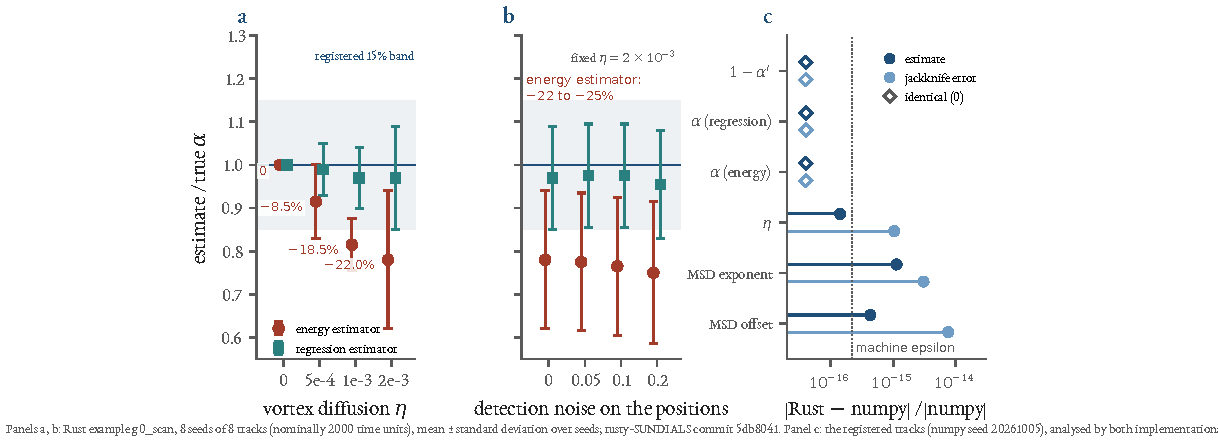
\includegraphics[width=\linewidth]{figures/ch10_estimator.pdf}
\caption[The energy estimator of the friction fails a known-answer test]{The energy estimator of the friction fails a known-answer test that it had passed once. \textbf{(a)}~Estimates divided by the true $\alpha=0.02$
as the diffusion $\eta$ of the model vortices grows, mean and standard deviation over \NxGateSeeds{} seeds of \NxGateTracks{} synthetic tracks
(Rust \texttt{g0\_scan}); the band is the registered 15~percent criterion. The identity of the theorem \texttt{energy\_dissipation} is exact
at $\eta=0$ and the energy estimator is exact there; the regression estimator stays near the truth. \textbf{(b)}~At $\eta=2\times10^{-3}$ the bias does not
depend on the detection noise added to the positions. \textbf{(c)}~The same eight tracks analysed by the numpy estimators and by the Rust estimators:
relative difference of every estimate.}\label{ch10:fig-estimator}
\end{figure}

Three things are visible in figure~\ref{ch10:fig-estimator}. First, in the noise-free model the energy estimator is exact (\NxGateEnergyZ{} against
$0.02$), as the theorem says it must be: the proved identity and the number agree where the hypothesis holds. Second, as soon as the vortices diffuse
the estimator is biased low, by \NxGateBiaseA, \NxGateBiaseB and \NxGateBiaseC~percent at the three diffusions tried, and the registered criterion
(within 15~percent) is met on only \NxQGatePassSeeds{} seeds in the programme's own count of this test; the gate had passed on, in the ledger's words,
``one lucky seed''. Third, the bias is not caused
by the detection noise: it is already there with none, and the energy estimator gives \NxGatenEnergyZ, \NxGatenEnergyA, \NxGatenEnergyB and \NxGatenEnergyC{} at
detection noise $0$, $0.05$, $0.1$ and $0.2$ per coordinate (panel~b). The regression estimator, which uses the same tracks, returns
\NxGateRegA, \NxGateRegB and \NxGateRegC{} at the same three diffusions and \NxGateOneminusapC{} for $1-\alpha'$ (truth $0.90$). Why the energy
estimator is biased we do not know. The programme's note suggests that the stochastic part of $H(t)$ is correlated with the cumulative regressor
$\int2\sum_i|\mathbf v_{s,i}|^2\mathrm dt$, which is computed from the same noisy path; that is a hypothesis, and is marked as one in the note.

Panel~(c) records what the second implementation did. The numpy estimators of the programme and the Rust estimators of \texttt{qf-pgpe} were run on
identical tracks and agree to \NxCrossMaxest{} in all six estimates and to \NxCrossMaxerr{} in their jackknife errors; on four real tracks the
software paper reports $2\times10^{-14}$ \cite{Callens2026sw}. On the registered tracks themselves (numpy seed 20261005), both implementations return $\alpha_{\rm energy}=\NxCrossEnergy$ --- the number with which the gate was recorded as
passed --- and $\alpha_{\rm regression}=\NxCrossReg$ with $1-\alpha'=\NxCrossOneminusap$. The agreement is the reason the Rust port could be trusted to expose a
defect, and the reason it could not have exposed this one by itself: two implementations of one estimator agree on its bias.

\subsection*{What it cost, and what it did not}

The programme's published friction values were computed with the energy estimator (CLAIM-098 of the ledger). The regression estimator is larger than the energy estimator by
$5$ to $21$~percent in the six measured arms, in exactly the direction of the bias, and the absolute values of $\alpha$ quoted in the first paper
\cite{Callens2026a} were therefore low by roughly \NxQBiasLo{} to \NxQBiasHi{}~percent. The coefficient of the temperature law
$\alpha/T$ rises from \NxQAlphatEnergy{} (energy) to \NxQAlphatReg{} (regression). The registered verdicts are comparisons between arms analysed with the same estimator, so none of them changes; both papers state the correction, the first in its results on the friction \cite{Callens2026a} and the second in its section on limits \cite{Callens2026b}.

\begin{keybox}[The rule]
A theorem is true of its hypotheses. Before an identity of the model is used as an estimator on data, test the estimator where the answer is known,
\emph{over many realisations}, and with the properties of the data (here: diffusion) switched on. This is the programme's rule LL-15 --- transfer a
result with its hypotheses, not just its conclusion --- applied to a theorem instead of to a measurement.
\end{keybox}

%=====================================================================================================================================
\section{What each check can and cannot see}\label{ch10:sec-checks}

The programme uses five kinds of check. Table~\ref{ch10:tab-checks} sets, for each, an instance in which it caught something and an instance, from
the same programme, in which it could not. None of the instances is hypothetical.

\begin{table}[tbp]\centering\footnotesize\renewcommand{\arraystretch}{1.15}
\begin{tabularx}{\linewidth}{@{}>{\raggedright\arraybackslash}p{0.14\linewidth}>{\raggedright\arraybackslash}X>{\raggedright\arraybackslash}X@{}}\toprule
check & caught, in this programme & could not see, in this programme\\\midrule
the Lean kernel and the axiom audit (Comparator: two kernels)
 & A count that had drifted: 76 theorems against 65 audit lines (RETRACTIONS.md, R3). A bug of the generator of the challenge files, which cut one
   statement at a \texttt{:=} inside a named argument, found while adding \brkident{SectorDuality} (CLAIM-052).
 & That the hypothesis of a true theorem fails in the data (section~\ref{ch10:sec-estimator}). That a true statement is empty: the dual-length bound is
   $x+1/x\ge2$ and ``could not have come out otherwise''. That a statement is the right physics: ``a Comparator pass says the solution proves the
   challenge's statement, not that the statement is the right physics'' (\brkident{docs/COMPARATOR\_SETUP.md}). That the hypotheses of a true theorem are met only by
   trivial cases: those of \texttt{KTFlow} (below, and \cref{ch06}).\\
a second implementation
 & A vortex centred on a grid node imprinted with modulus one instead of zero, in the first Rust version. A defect of the Adams order in the CVODE
   library, exposed by the first Hamiltonian system run through it. The estimator bias, once a seed sweep was cheap.
 & An error shared by both: numpy and Rust agreed to $2\times10^{-14}$ on four real tracks and both were biased. A platform effect that
   one platform hides: a $T=0$ control run that agrees to $10^{-13}$ on x86-64 differed by $8\times10^{-3}$ in position on an Apple-silicon runner.\\
a registered test
 & \NxVerdNotmet{} of \NxVerdCells{} criteria not met (figure~\ref{ch10:fig-verdicts}), each against a threshold written down beforehand.
 & A criterion that cannot fail for the reason intended: the residual criterion D-G2$''$ was ``mis-specified, since the vortex term is 500$\times$ the
   phonon term''. A battery of six criteria that all tested deterministic reproducibility in a chaotic model and none statistical reproducibility (LL-14).\\
the solver library's own tests
 & Nine tests of the Adams method of CVODE, written \emph{before} the fix of its defect (the method was implicit Euler); eight of them fail on the
   unfixed code (\brkident{crates/cvode/tests/adams\_order.rs}, \brkident{docs/CVODE\_ADAMS\_FIX.md}).
 & Which binary a script imports. The Python module installed in the shared environment of this book was built on 26~September, before the fix of 28~September:
   $y'=-y$ to $t=10$ at relative tolerance $10^{-10}$ cost \NxCvodeStaleNfe{} right-hand-side calls and returned an error of $\NxCvodeStaleErr$, against
   \NxCvodeFixedNfe{} calls and $\NxCvodeFixedErr$ for the build of commit 5db8041. The tests had run on the source. A convergence check in a chapter found the stale
   binary; no test did.\\
independent data
 & Two facts about a published reference run, found by trying to reproduce it: an $O(\Delta t)$ convention in its velocity ramp, and an initial field that
   is the Thomas--Fermi field after one imaginary-time step plus noise (the stopping rule is met at the first step).
 & Anything beyond the window reproduced: not $t>50$, not the Strouhal number, not single precision against discretisation; the model had to be recovered
   from the code, not from the paper's text.\\\bottomrule
\end{tabularx}
\caption{Five kinds of check, each with an instance of what it caught and of what it missed. Sources: RETRACTIONS.md, LEDGER.md (CLAIM-052, 079, 092, 098,
103, 106), LL.md (LL-14), the software paper \cite{Callens2026sw}, \texttt{docs/CVODE\_ADAMS\_FIX.md} of rusty-SUNDIALS, and the probe of appendix~\ref{appB}.}\label{ch10:tab-checks}
\end{table}

Two observations. The checks are not ordered by strength: each answers a different question --- is the statement what we think it is, does the code
compute what its author intended, does the binary that runs contain that code, was the verdict chosen before the data, does anyone else's data agree --- and
passing one is silent about the others. And a check is credited only when it has been \emph{run}. The programme's habit, visible in every row of the table, is to ask of a result
\emph{which} of these it has passed, and to write the answer down before anyone cites the result.

%=====================================================================================================================================
\section{The audit of the library}\label{ch10:sec-audit}

A sentence such as ``the library has \NxLibThm{} theorems, none uses \texttt{sorry}, all use only the three standard axioms'' is a claim about a
build, and it can be checked only by building. The programme's records show how easily it drifts. In September an external review of the v1.1.0
tag found that \brkident{DualLength.lean} declared 13 theorems while the reported count was 12; looking at all the files showed that \NxQRThreeListed{}
theorems existed where \NxQRThreeAudited{} carried a \texttt{\#print axioms} line, so \NxQRThreeMissed{} had never been audited and every published count
had conflated ``theorems'' with ``theorems carrying an audit line'' (RETRACTIONS.md, R3). The repair was a generator, \brkident{scripts/regen\_axiom\_audit.py},
which rewrites the audit block of every file and has a read-only \texttt{--check} mode.

For this book we audited the library again, differently. The driver (appendix~\ref{appB}; \brkident{book/facts/lean\_audit.py}) compiles each module,
in the order of its imports, against the pinned Mathlib (Lean 4.34.0-rc2, Mathlib tag v4.34.0-rc2), after appending to a scratch copy about twenty
lines of Lean --- new for this book, printed in appendix~\ref{appB} --- that walk the kernel environment of the module, ask \brkident{Lean.collectAxioms}
about \emph{every constant the file declares}, and print the union. It audits the environment, not the text: it needs no \texttt{\#print axioms} line
in the source. Like any auditor it has to be seen to catch something. Run on a file with planted defects it reports a \texttt{sorry}, the
same \texttt{sorry} inherited by a theorem whose own proof contains none, a \texttt{sorry} in a private theorem, an axiom declared by the module and
a use of \brkident{native\_decide}, and it reports the clean theorems as using at most \texttt{propext}, \brkident{Classical.choice} and \texttt{Quot.sound}
(\brkident{facts/audit\_controls/}). A grep for the word \texttt{sorry} in the compile log finds two of the three theorems that depend on a \texttt{sorry}; the third has no warning of its own.

\begin{figure}[!t]\centering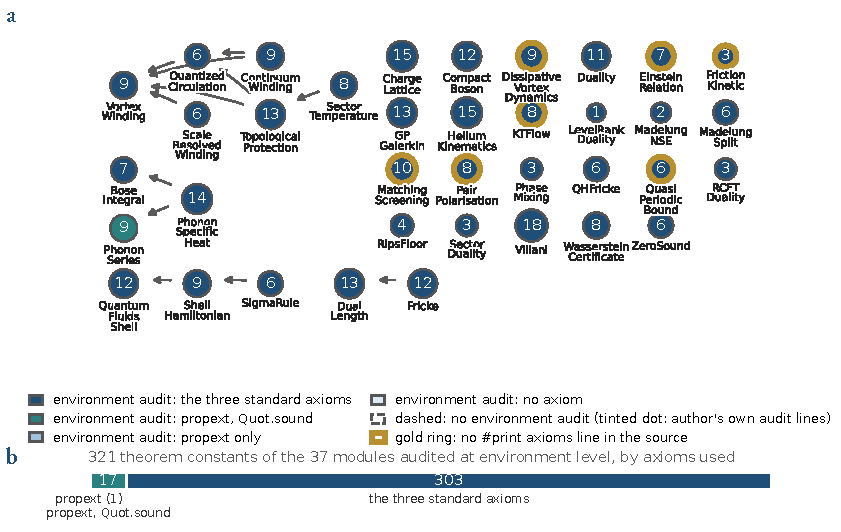
\includegraphics[width=\linewidth]{figures/ch10_library.pdf}
\caption[The library as audited for this book]{The library as audited for this book. \textbf{(a)}~The \NxLibModules{} modules, placed by the import relation (arrows point from a module to
the modules it imports), the size of a disc growing with the number of theorems of the module (printed inside); fill = the axiom footprint found by the environment audit, a dashed outline = no current
environment audit (\NxLibUnaudited{} when the figure was drawn), a gold ring = the module's source carries no \texttt{\#print axioms} line of its own (\NxLibNoprint{} modules). \textbf{(b)}~The axiom footprint of every theorem constant of
every module, from the environment audit.}\label{ch10:fig-library}
\end{figure}

\paragraph{What the audit found.} Five things are worth telling.

\emph{The first run of our own driver reported nine failures, and none was real.} It compiled each file separately, inside the Mathlib tree; nine
modules import a sibling (\texttt{import VortexWinding}) whose compiled file was not on that tree's search path, so Lean answered \texttt{unknown
module prefix}. The driver of this book builds in dependency order and puts the compiled siblings on the path.

\emph{Seven modules carry no \texttt{\#print axioms} line}, and their compile logs are therefore empty: \brkident{DissipativeVortexDynamics},
\brkident{EinsteinRelation}, \brkident{FrictionKinetic}, \texttt{KTFlow}, \brkident{MatchingScreening}, \brkident{PairPolarisation} and
\brkident{QuasiPeriodicBound}. An empty log of a module that compiles is not a timeout and not a failure; it is a module that was never asked. Asked (table~\ref{ch10:tab-seven}), each of the seven
compiles without error and depends on at most the three standard axioms; no \texttt{sorry} is reachable from any of their \NxAuditSevenThm{} theorems.
The staleness check introduced after R3 (\texttt{python3 scripts/regen\_axiom\_audit.py --check}, read-only) flags exactly these seven library modules (and four scratch files): the drift that R3
repaired reappeared within three weeks of its repair, for the same reason: the check exists, and no script, workflow or git hook of the repository calls it. The programme's gate
script \brkident{scripts/verify.sh} builds a single module (\brkident{QuantumFluidsShell}) and searches the log for \texttt{sorryAx}. The same seven
modules are also the ones that the Comparator list (\NxLibCmpModules{} modules, \NxLibCmpThm{} theorems, accepted by the Lean kernel and by
nanoda \cite{LeanComparator,Nanoda}) does not contain.

\InputIfFileExists{figures/ch10_audit_seven}{}{}

\emph{The generator that repaired the count has a blind spot of its own.} It recognises a theorem only at the start of a line, so
\brkident{crossover\_apply\_mem} and \brkident{crossover\_apply\_not\_mem} in \texttt{Villani.lean}, declared as \texttt{@[simp] theorem}, were never given an
audit line: the generator counts \NxLibGenThm{} theorems where the index of the library lists \NxLibThm{}. The generator of the Comparator's challenge files keeps the
theorems that carry an audit line, so it inherits the blind spot: the \NxLibCmpThm{} theorems that the Comparator accepted are the \NxLibCmpGen{} listed ones, out of
\NxLibCmpIdx{} in the thirty modules it covers (the two missing are the two above). \NxVillaniSimp

\emph{One module is outside the build.} \brkident{FrictionKinetic.lean} appears neither in \brkident{lakefile.lean} nor in the umbrella file
\brkident{QuantumFluids.lean}: \texttt{lake build} does not build it, and \texttt{import QuantumFluids} does not give its theorems.

\emph{The index of the library, from which this book's citations of theorems were first taken, was wrong about the names.} It said that every module lives in
the namespace \brkident{QuantumFluids.}\emph{Module}. For \NxLibOddNs{} of the \NxLibModules{} modules it does not: the seven newest modules sit in bare namespaces
(\brkident{KTFlow.kt\_trapped}), \texttt{Duality} sits in \brkident{Mathesis.Duality}, \brkident{QuantizedCirculation} in \brkident{QuantumFluids.Circulation},
and \brkident{QuantumFluidsShell}, \brkident{ShellHamiltonian} and \texttt{SigmaRule} in \brkident{QuantumFluids.ShellComplex}. The error was found only when the
catalogue of appendix~\ref{appA} was generated from the sources instead of typed, and the book's theorem-citation macro now looks the namespace up.
It is the same kind of error as the drifting count: a statement about the library that nobody had compared with the library.

\emph{The result.} \InputIfFileExists{figures/ch10_audit_result}{}{\textbf{[The environment audit had not finished when this text was generated; the sentence that reports it is written by \brkident{figures/ch10\_audit\_text.py} once the audit is complete.]}} \InputIfFileExists{figures/ch10_audit_book}{}{}

\paragraph{What the audit does not do.} It reads the environment that Lean's elaborator produced and trusts Lean's kernel; the second kernel is the
Comparator's business, and we did not re-run Comparator for this book (its results are those recorded in \brkident{docs/COMPARATOR\_SETUP.md}). It says
nothing about whether a statement is the right one; the statements are in appendix~\ref{appA} for a human to read, and a Comparator pass shows the same statement only because, in the words of the programme's own note,
``\,`same statement' is guaranteed by construction'' when the challenge file is generated from the solution. And it is only
as complete as the list of modules: the umbrella file and the lakefile are part of what has to be kept in step.

%=====================================================================================================================================
\section{What failed, plainly}\label{ch10:sec-failures}

The ledger of the programme (\texttt{LEDGER.md}) numbers its claims; in \NxLedgerDays{} days, from \NxLedgerFirst{} to \NxLedgerLast, it reached
claim \NxClaimsLast. Its entries carry statuses, and a good many of the statuses are the words \emph{retracted}, \emph{withdrawn}, \emph{refuted} or
\emph{void}. Only \NxClaimsChecked{} of the \NxClaims{} claims are in the format that the ledger's own checker (\brkident{scripts/check\_ledger.py})
reads; the rest are in a second, tabular format that it does not see --- a limitation of the machine check that the ledger itself records (CLAIM-066).
What follows is therefore a reading of the text, not a statistic.

\paragraph{A map of the verdicts.} Figure~\ref{ch10:fig-verdicts} draws every criterion that the ledger records one by one, for \NxVerdRows{} of the
programme's campaigns. There are \NxVerdCells{} of them: \NxVerdMet{} were met as registered, \NxVerdNotmet{} were not, \NxVerdMixed{} were mixed, partial
or inconclusive, one was voided afterwards and one was not run. The criteria are not independent and not equally important --- the kinetic benchmark
contributes $25$ cells, the finite-size ladder $7$ --- and the selection rule is the only one available to us: the campaigns whose per-criterion
outcomes the ledger gives. It shows how often a criterion written down before the data was not met, among those the ledger itemises: nearly as often as it was met.

\begin{figure}[tbp]\centering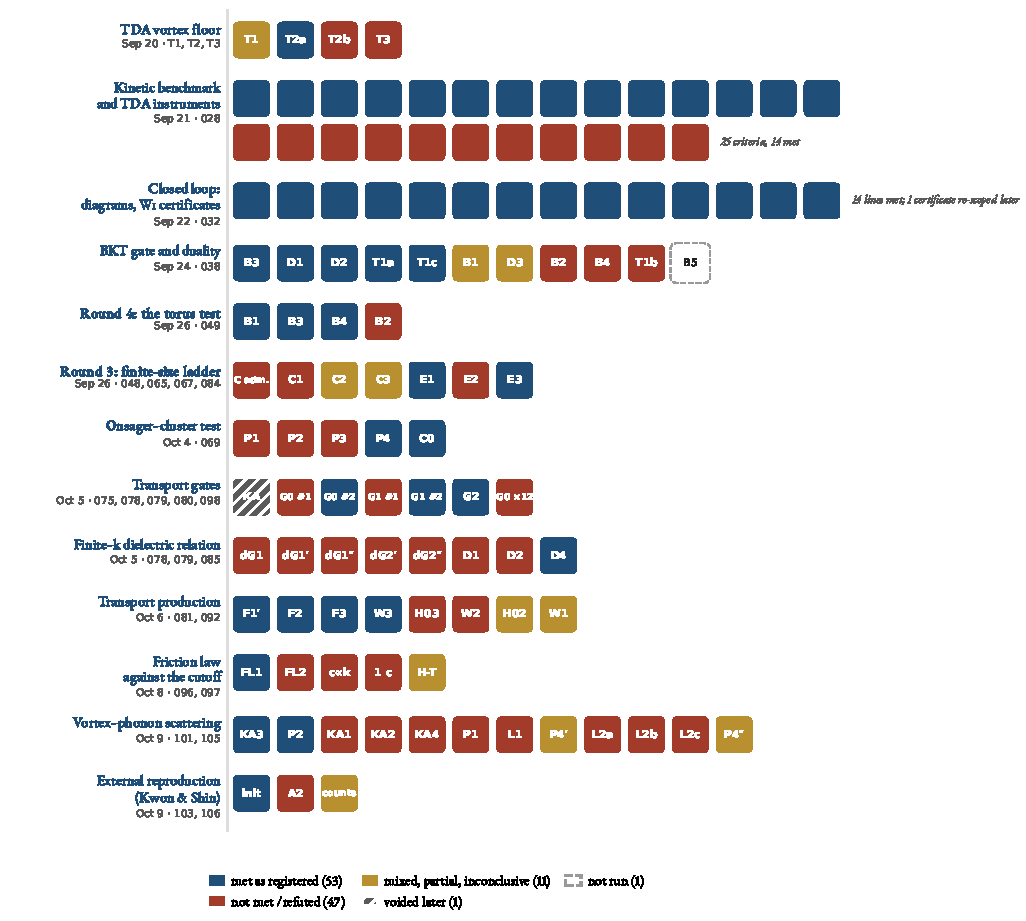
\includegraphics[width=\linewidth]{figures/ch10_verdicts.pdf}
\caption[Every criterion the ledger records, by campaign]{Every criterion that the ledger records one by one, by campaign (numbers are ledger claims; figure script \texttt{figures/ch10\_verdicts.py}
checks each row against \texttt{LEDGER.md}). Blue: met as registered; red: not met or refuted; gold: mixed, partial or inconclusive; hatched: voided
afterwards; dashed: not run. Unlabelled cells are criteria the ledger counts but does not name. Labels are those of the registration documents:
for instance P1--P3 are the registered predictions of the Onsager-cluster test (all three failed), G0/G1 the gates of the transport campaign (each
failed at its first attempt), D1/D2/D4 the criteria of the dielectric test, FL1/FL2 those of the friction-law test, L1/L2a--c those of the
vortex--phonon scattering test. The cell \emph{G0$\times12$} is the energy criterion of G0 re-run over many seeds (section~\ref{ch10:sec-estimator}).}\label{ch10:fig-verdicts}
\end{figure}

\paragraph{September: the literature check.} On 20~September the programme pre-registered a hypothesis, the \emph{dual scale} of a quantum fluid,
stated it in Lean, and refuted it for helium~II by measurement; the release of that day is tagged ``stated, proved, and refuted for He-II''. The same
day the literature check that the proposal itself had listed as blocking any claim of novelty was run, and it went against the programme on both
counts (RETRACTIONS.md). The second invariant of the complexified shell model was a rediscovery of structures in Vladimirova, Shavit and Falkovich's
\emph{Fibonacci turbulence} and in a second paper by overlapping authors on second-harmonic generation as a minimal model of turbulence
\cite{Vladimirova2021a,Vladimirova2021b}; on the dyadic lattice the family of conservation laws collapses to a single invariant, so the model has
\emph{less} structure than the published one. The dual length $\ell(k)=\varepsilon^2/(\hbar^2c^2k^3)$ was a repackaging of the static response, its
``bound'' was the inequality between the arithmetic and the geometric mean, it was weaker than the known linear bound of Onsager's inequality
\cite{WreszinskiDaSilva2005} outside a narrow window of wavenumbers, and its interior minimum was dimensionally forced; the ``refutation'' for helium
was structural, since any fluid with a roton violates it. The file states the outcome in one sentence: ``No novel scientific contribution survives
in the dual-scale programme.'' What survived were the Lean proofs, as correct mathematics of known results, the measurements, as correct measurements
of textbook physics, and a record of method. The same file lists a repository defect (a symlink to a local disk, committed by mistake, which broke every
clone) and the counting error of section~\ref{ch10:sec-audit}.

\paragraph{Failures of our own design.} Not every failure came from outside. Lessons LL-7 to LL-14 of the programme's \texttt{LL.md} record
what the first weeks cost. A table of literature constants entered the roton gap in kelvin and used it as millielectronvolts, overstating it by the
Boltzmann-constant factor, about $11.6$, and a conversion constant was off by exactly $2$; the synthetic tests had been generated with the same wrong
constants they checked, and both errors surfaced only against real, digitised data (LL-7). Values of the phonon--roton (Landau) parameters recalled from memory were attributed to two
papers that report no such values; they were within about $0.3$~percent of the true ones, which is why they survived (LL-10). An exponent fitted to the
supremum of the enstrophy was a property of the horizon chosen, because the supremum does not converge in the horizon for a conservative regulator,
and every quality signal --- $r^2>0.96$, disjoint confidence intervals, a timestep-refinement criterion passing at $0.00$~percent --- was good (LL-11).
The thermalisation time of the chaotic model has a coefficient of variation of $23$ to $49$~percent from one realisation to another at fixed parameters, and four rounds
of results had come from a single trajectory (LL-14). And a lesson that is not about physics: a destructive check of the Lean gate, which inserts a
\texttt{sorry} into a source file, was launched as one background command, outlived its foreground timeout, and the file still contained the
\texttt{sorry} when a commit was being prepared; ``the margin was one grep'' (LL-13).

\paragraph{October: the campaign.} The pre-registered campaigns of October produced most of the cells of figure~\ref{ch10:fig-verdicts}, and the
ledger reads like a lab book of an apparatus that did not work the first time. The friction known-answer gate of CLAIM-075 was recorded as passed on 5~October
and withdrawn the same day, when the first gates of the transport campaign were run, because the vortex imprint of the instrument added an amplitude tail four times the Bernoulli depletion and a phase step
along a whole line of the box, and the apparent friction at $T=0$ was as large as the thermal value being measured (CLAIM-078). The counterflow control
W2 was refuted, one run of four meeting the no-stall criterion (CLAIM-092). The friction law ``$\alpha\propto\rho_n$'' was found to be a degeneracy of
one cutoff, since $\rho_n\propto T$ there; across three cutoffs the coefficient is $0.31$, $0.23$ and $0.10$ and only $\alpha/T$ is constant
(CLAIM-096), and the paper that had published the first reading, together with a ``geometric core size of $1.4\,\xi$'' derived from it, had to be corrected in
version 2.2. The finite-k dielectric relation, tested mode by mode, held in one run of six; an earlier correlation of $0.996$ across runs had been carried by
box-scale pairs (CLAIM-085). The vortex--phonon scattering cross-section depended on the pair separation and on the box, and the registered conclusion is that an
isolated-vortex $\sigma_\parallel(k)$ ``is not defined by this observable at these geometries'' (CLAIM-105).

Two failures were failures of process rather than of physics. A verdict of ``saturation'' for the finite-size offset at $L=192$ (CLAIM-067,
admission $3$ of $6$) was recorded as unresolved, and a longer run (CLAIM-084, admission \NxQCFourAdm) showed that it had rested on states that had not
equilibrated; the finite-size trend of the whole ladder was then, in the ledger's words, under the same suspicion. And the first Python attempt
at those $L=192$ runs died silently after about \NxQCThreeHours{} hours, with nothing in its log; the cause could not be diagnosed, an out-of-memory
kill being ``the leading, unconfirmed hypothesis''. The runs were redone with a Rust port of the integrator, which itself stopped once without an error
and was resumed from a checkpoint.

A third process failure happened while this book was being written. The Python module \brkident{rusty\_sundials} installed in the shared environment had been built on
26~September (the stale module of the probe of appendix~\ref{appB}), two days before the Adams method of the solver library was repaired; in that build the method is implicit
Euler, and its work grows like $\mathrm{rtol}^{-1/2}$. The library's tests, written before the repair, fail on the old code, but they test the source, not the file that a script imports.
The defect was caught by a convergence check in one chapter. The probe of appendix~\ref{appB} (Adams on $y'=-y$ to $t=10$ at relative tolerance $10^{-10}$) separates the two
builds: \NxCvodeStaleNfe{} right-hand-side calls and an error of $\NxCvodeStaleErr$ before, \NxCvodeFixedNfe{} calls and $\NxCvodeFixedErr$ after. No computation of
this chapter used CVODE through that module; the lesson is the one of section~\ref{ch10:sec-estimator} applied to a binary: a check certifies the thing it was run on.

\begin{table}[tbp]\centering\small\renewcommand{\arraystretch}{1.12}
\begin{tabularx}{\linewidth}{@{}>{\raggedright\arraybackslash}p{0.11\linewidth}>{\raggedright\arraybackslash}p{0.27\linewidth}>{\raggedright\arraybackslash}X>{\raggedright\arraybackslash}X@{}}\toprule
when & what was withdrawn or corrected & what had failed & rule or repair\\\midrule
Aug 14--15 & exponent comparison, ordinal-censoring result (CLAIM-R1, R2, 012, 013) & horizon not converged; one trajectory of a chaotic system & LL-11, LL-14: converge in the horizon; measure the ensemble spread first\\
Aug & prediction exported to a sister project (CLAIM-017) & tested in their code before it was sent: exponent stable to four decimals over $8\times$ horizons & LL-15; retracted the same turn\\
Sep 20 & second invariant, dual length, $\sigma$-rule (CLAIM-023, 024, 025) & rediscovery; weaker than the known bound; dimensionally forced & RETRACTIONS.md; no novelty claimed\\
Sep 20 & TDA vortex floor (CLAIM-T1, T2, T3) & confounded by the segmentation threshold; split verdict; refuted & threshold-free line tracing; ``nothing from this run is citable''\\
Sep 21 & kinetic benchmark and TDA instruments (CLAIM-028) & \NxQKinNot{} of $25$ criteria not met; Lean formalisation of nonlinear Landau damping called ``out of reach'' six days after it had been posted \cite{Bedrossian2026} & literature gate before any claim of difficulty\\
Sep 22 & Wasserstein certificate, phase-space pair (CLAIM-032 erratum) & computed on $5$ points per side instead of the registered $30$; the same class of defect as a point list changed between workflow stages, found the same day & all pairs recomputed independently; erratum carried into the next paper\\
Oct 5 & friction known-answer gate (CLAIM-075 $\to$ 078) & imprint with an amplitude tail and a phase step & new imprint; gates G0--G2\\
Oct 8 & counterflow control W2 (CLAIM-092, 095) & $1$ of $4$ runs met the criterion; a template-filled paragraph contradicted the verdict & explanation withdrawn, observation kept; text corrected\\
Oct 8--9 & $\alpha\propto\rho_n$ and a core size of $1.4\,\xi$ (CLAIM-096, 099) & coefficient depends on the cutoff; $\rho_n\propto T$ degeneracy & paper corrected (v2.2); $\alpha/T$ reported\\
Oct 9 & energy estimator of $\alpha$ (CLAIM-098) & biased low by diffusion; gate passes on $2$ of $12$ seeds & regression estimator; gates run over seeds\\\bottomrule
\end{tabularx}
\caption{What was withdrawn or corrected, why, and the rule or repair that followed. Every row is an entry of \texttt{LEDGER.md}, \texttt{RETRACTIONS.md} or
\texttt{LL.md}.}\label{ch10:tab-failures}
\end{table}

\paragraph{Two statements that stayed true.} Not everything in the middle of a failed campaign fails. Two Lean statements of the transport campaign
illustrate what a proved statement does \emph{not} change.

\begin{leanbox}{QuasiPeriodicBound}
\begin{lstlisting}[style=lean]
noncomputable def qp (a ω φ : ι → ℝ) (t : ℝ) : ℝ := ∑ k, a k * Real.cos (ω k * t + φ k)

theorem not_qp_of_msd_large (a : ι → ℝ) {J : Type*} [Fintype J] [Nonempty J] (x : ℝ → ℝ) (ts τs : J → ℝ)
    (h : (2 * ∑ k, |a k|) ^ 2 < (∑ j, (x (ts j + τs j) - x (ts j)) ^ 2) / Fintype.card J) :
    ∀ ω φ : ι → ℝ, x ≠ qp a ω φ
\end{lstlisting}
\end{leanbox}

\noindent The first is the logic of a discriminant. A vortex pair whose motion is a regular island has quasi-periodic coordinates, finite sums of cosines;
the statement says that if the sampled mean-square increment of a signal exceeds $(2\sum_k|a_k|)^2$, the signal is not such a sum for \emph{any}
frequencies and phases with those amplitudes. The docstring is explicit that the decision rule is ``sound in one direction and silent in the other'': growth
refutes the island reading, a plateau proves nothing. On the data the registered criterion I2 was read as ``not an island'' --- the separations of the
stalled pairs carried a third of their variance in their three largest spectral lines, less than the registered half (CLAIM-086) --- and nothing about the
statement had to be revised.

\begin{leanbox}{FrictionKinetic}
\begin{lstlisting}[style=lean]
noncomputable def alpha (K : Finset ι) (w f : ι → ℝ) (ρs κ : ℝ) : ℝ := (∑ k ∈ K, w k * f k) / (ρs * κ)

noncomputable def rhoN (K : Finset ι) (w : ι → ℝ) : ℝ := ∑ k ∈ K, w k

theorem coeff_eq_weighted_mean (K : Finset ι) (w f : ι → ℝ) (ρ ρs κ : ℝ) (hρn : rhoN K w ≠ 0) (hρ : ρ ≠ 0) :
    alpha K w f ρs κ / (rhoN K w / ρ) = ρ / (ρs * κ) * ((∑ k ∈ K, w k * f k) / ∑ k ∈ K, w k)
\end{lstlisting}
\end{leanbox}

\noindent The second is an identity of a kinetic model of the friction: if the drag and the normal density are sums over the same bath modes $k\in K$ with the
same nonnegative weight $w_k$, the drag carrying one more factor $f_k$ (group velocity times transport cross-section), then the ratio $\alpha/(\rho_n/\rho)$
is a constant times the $w$-weighted mean of $f$ over the modes (the proof is algebra: abridged here). What the statement says about the world is only
that this coefficient is a property of the \emph{bath}: it can depend on the modes retained. It does not say that it is independent of the cutoff, and when
the registered expectation that it nearly is (spread below $0.2$) failed --- the coefficient was $0.31$, $0.23$ and $0.10$ at the three cutoffs --- the
identity was not affected. What was withdrawn was a reading of the number measured at one cutoff, a ``geometric core size of $1.4\,\xi$''. The theorem
is a statement about the model, the $1.4\,\xi$ was a statement about the world, and only the first had been proved.

\paragraph{A statement that was true and nearly empty.} A third statement was true, and its trouble was of the opposite kind: in the estimator story a hypothesis failed in the data, here a hypothesis
can hardly be met by anything. It was found while \cref{ch06} was being prepared. Three theorems of \texttt{KTFlow} (\Lthm{KTFlow}{kt_invariant}, \Lthm{KTFlow}{kt_trapped} and
\Lthm{KTFlow}{kt_fugacity_bounded}) are about a solution $(u,y)$ of the Kosterlitz flow, and the file asks for the two flow equations and for $u>0$ \emph{at every real
scale} $l$, negative ones included (the hypotheses \texttt{hu}, \texttt{hy} and \texttt{hpos} are quantified over all $l\in\mathbb R$), whereas a renormalisation
trajectory is a solution for $l\ge0$ only. \Cref{ch06} proves, in a new module of the book, that on the superfluid side these hypotheses leave almost nothing: if
$u(0)<\pi/2$ then $y(0)=0$. (If $y(0)\neq0$, the invariant forces $y(l)^2\ge y(0)^2$ for $l\le0$, so going backward $u$ would fall at least linearly and be negative
before $l=-u(0)/c$, with $c=4\pi^3y(0)^2$, which the hypothesis $u>0$ forbids.) From $y(0)=0$ the uniqueness of the solution of the linear equation for $y$ gives
$y\equiv0$ and $u$ constant --- a standard step, not formalised --- so only fixed points of the flow meet the hypotheses there. The three theorems are true, and the
kernel certified exactly what had been written; what had been written asked too much of a solution to be applied to one that matters. The library file is unchanged; \cref{ch06} restates the theorems under hypotheses on
$l\ge0$ only, and adds the converse.

\paragraph{A name that was copied, not checked.} The 2021 paper of Godfrin and his co-authors \cite{Godfrin2021} has seven authors. While this book was written its
record at the publisher (Crossref) was compared with the programme's own notes, and two of them gave the list wrongly: the literature ledger wrote the second
author's initial as M instead of K, and a design note, like the docstring of the library module \brkident{PhononSeries}, named an eighth author who is not on the paper.
No test could catch a name, and none did; the slips were found by looking the record up. They were corrected on 10~October 2026 (in the library the change is a
comment, so no theorem is touched); the copy of that module that is generated for the Comparator repeats the old docstring until its generator is run again.
It is the lesson of the other paragraphs at the smallest scale: a copy of a copy is not a source.

\paragraph{What the failures have in common.} The following is our reading, not a measurement. Most of the entries of table~\ref{ch10:tab-failures}
fall into three kinds: a result used outside the hypotheses on which it depended (the estimator; the prediction exported to a sister project; the
friction law outside one cutoff); one realisation mistaken for an ensemble (the single trajectories of August, the single seed of G0, a single seed
per energy at $L=192$); and a gate or a criterion that could not fail for the reason intended (the battery of LL-14, the imprint that made the
known-answer gate pass, the residual criterion D-G2$''$). They are the same three mistakes at three scales, and each has a cheap check, which is
what the rules of the programme are: write down the hypotheses and check them in the target (LL-15), measure the spread before fitting (LL-14),
and run the gate where the answer is known with the property switched on (section~\ref{ch10:sec-estimator}). They are also the reason that pre-registration
\cite{Nosek2018} is only half a method: a registered criterion makes the verdict impossible to bend, and does nothing about whether the criterion could
have failed for the right reason.

%=====================================================================================================================================
\section{Speed is a claim too}\label{ch10:sec-speed}

The solver of this book is offered as a tool, and a tool has a speed; claims of speed are checked less often than claims of physics. The benchmark of
the software paper \cite{Callens2026sw} times one step of the projected Gross--Pitaevskii integrator on an $N\times N$ grid ($L=N/2$, $g=1$,
$\Delta t=0.01$), identical in every engine; the final states agree in a checksum (to \NxBenchJaxchk{} for JAX against Rust), so the timings are for the same computation.

\begin{figure}[!t]\centering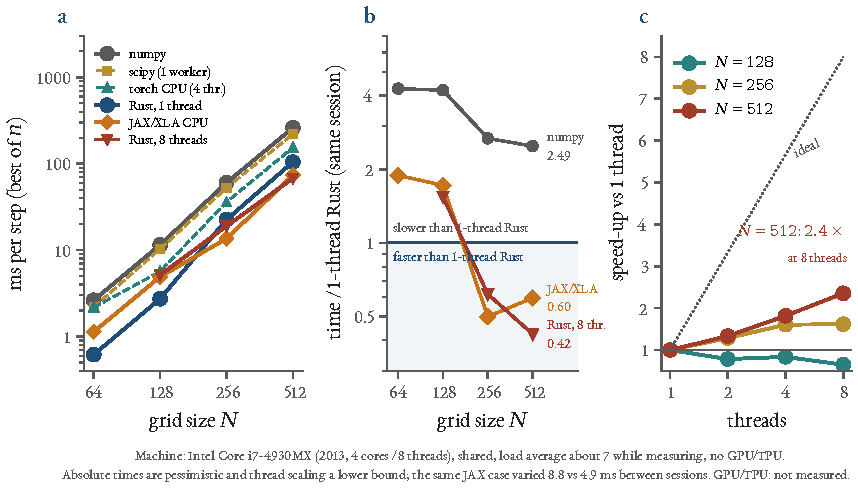
\includegraphics[width=\linewidth]{figures/ch10_bench.pdf}
\caption[Time per step of the projected Gross--Pitaevskii integrator in several engines]{Time per step of the projected Gross--Pitaevskii integrator in several engines (best of $n$ repetitions). \textbf{(a)}~Absolute time against grid size
$N$. \textbf{(b)}~Time relative to the one-thread Rust step measured in the same session, so that load common to both cancels in part; values below one
are faster than serial Rust. \textbf{(c)}~Speed-up of the threaded Rust step against its own one-thread time. All measurements were taken on one shared
machine (Intel Core i7-4930MX, 2013, 4 cores and 8 threads, load average $\approx7$, no GPU); the same JAX case gave $8.8$~ms in one session and
$4.9$~ms in another. Data: \texttt{data/generated/pgpe/bench/}.}\label{ch10:fig-bench}
\end{figure}

On one thread the Rust engine takes \NxBenchRustA, \NxBenchRustB, \NxBenchRustC{} and \NxBenchRustD~ms per step at $N=64$, $128$, $256$, $512$, against
\NxBenchNumpyA, \NxBenchNumpyB, \NxBenchNumpyC{} and \NxBenchNumpyD~ms for numpy: \NxBenchSpnpA, \NxBenchSpnpB, \NxBenchSpnpC{} and \NxBenchSpnpD{} times faster,
the advantage shrinking with $N$. A JAX/XLA version on the CPU is slower than serial Rust at $N=64$ and $128$ and faster at $N\ge256$; pinned to one core
the order reverses, so the XLA lead at large $N$ is threading and not a better algorithm. Threading the Rust step helps at $N\ge256$
(\NxBenchThrBig$\times$ at $N=512$ on eight threads, \NxBenchThrMid$\times$ at $N=256$) and \emph{hurts} at $N=128$:
\NxBenchSmallEight~ms on eight threads against \NxBenchSmallOne~ms on one, so for small grids the threading must stay off.

What is not claimed matters as much. There is no comparison with FFTW-based C codes, with GPU codes or with any other published solver, and no
measurement on a GPU or a TPU; the machine was shared, so absolute times are pessimistic and the scaling is a lower bound; the statistic is the best
of a few repetitions, taken in the same way for every engine, in two sessions that differ by up to a factor of two for the same case. ``Fast'' in this
book means ``faster than numpy on this machine, for this problem, on one thread''. It does not mean ``the best solver''.

%=====================================================================================================================================
\section{What a reader can reuse}\label{ch10:sec-legacy}

\paragraph{The library.} The Lean library \cite{Callens2026lib} is \NxLibModules{} modules and \NxLibThm{} theorems and lemmas, with \NxLibDef{} definitions,
structures and abbreviations (catalogue in appendix~\ref{appA}). It is pinned to Lean 4.34.0-rc2 and to the Mathlib tag of the same name, and is licensed
MIT or Apache-2.0. A reader who wants a result, rather than a method, should look first at the modules whose subject is mathematics with a physical
reading: \texttt{BoseIntegral}, \texttt{PhononSeries} and \brkident{PhononSpecificHeat} (the coefficients of the phonon specific-heat series),
\texttt{ZeroSound} (when an undamped zero-sound root exists), \brkident{VortexWinding} and \brkident{QuantizedCirculation} (that the way simulation codes find
vortices measures an integer), \texttt{KTFlow} (the Kosterlitz renormalisation flow). Every module is a top-level module of its own: the umbrella file
\brkident{QuantumFluids} imports all but one.

\begin{godfrinbox}{the series of Eq.\,(22), and a remark of its authors}
In the paper on the dispersion relation of the Landau excitations of superfluid $^4$He, measured by inelastic neutron scattering on IN5 at the ILL,
Godfrin and co-authors give in Eq.\,(22) the phonon specific heat $C_V=AT^3+CT^5+DT^6+ET^7+KT^8+LT^9$ for a dispersion
$\varepsilon=\hbar ck(1+\alpha_2k^2+\dots+\alpha_6k^6)$ with $\alpha_1=0$, and remark that earlier published versions of this series contain
errors \cite{Godfrin2021}. The library has derived the six coefficients independently (with sympy) and proved them in Lean
(\texttt{BoseIntegral}, \texttt{PhononSeries}, \brkident{PhononSpecificHeat}): a confirmation of the paper's Eq.\,(22), not a finding. What is proved is
the mathematical statement, a series coefficient; it is not a statement about the experiment.
\end{godfrinbox}

A series of six terms, each a polynomial in the coefficients of the dispersion relation, is algebra that a machine can check at small cost; but the
same remark applies to it as to everything above: the kernel certifies the algebra, and the physics of the dispersion relation is in the measurement.

\paragraph{The solver.} The engine \texttt{qf-pgpe} of rusty-SUNDIALS (release v11.6.0; software paper \cite{Callens2026sw}) is a pure-Rust
projected Gross--Pitaevskii integrator with a Python extension, \texttt{qf\_pgpe}, whose \texttt{Pgpe}, \texttt{imprint\_v2}, \texttt{detect} and
\brkident{analyse\_tracks} are drop-in replacements for the numpy versions of the programme; CVODE \cite{Hindmarsh2005} is available through
\brkident{rusty\_sundials} (take the build of commit 5db8041 or later, and check it with the probe of appendix~\ref{appB}). What is reusable beyond the code is the
verification harness: the cross-language comparison on identical inputs, the CVODE reference, run with the repaired Adams method, that confirms the fourth order
of the step, and a reproduction test of the Kwon and Shin run \cite{KwonShin2026data} on its real download,
which runs weekly and on demand outside the required checks (\cref{ch09}).

\paragraph{The discipline.} It is the part of the programme that held up under its own failures, and it is small enough to list.
\begin{keybox}[A checklist, from the programme's practice and from the making of this book]
\begin{enumerate}[nosep,label=\arabic*.]
\item Register the criteria, the decision rule and the kill rule \emph{before} the data exist, in a file under version control \cite{Nosek2018}.
\item Give every instrument a known-answer test, run it over many realisations and with the property of the data that will matter switched on.
\item Have a second implementation, or a second source of data, for every number that will be quoted.
\item Write down the hypotheses of a result before exporting it, and test each in the target (LL-15).
\item Give every constant that stands for a measurement its source, table and uncertainty in a comment beside it (LL-10).
\item Read the literature for the claim of novelty \emph{and} for the claim of difficulty before either is made.
\item Keep a ledger with statuses that include \emph{refuted} and \emph{withdrawn}, and correct a published number in the next version of the paper that
 carries it.
\item Look a citation up in the publisher's record before it is printed; a copy of a copy is not a source.
\item Make the record reproducible from files: a script for every figure, a source for every number (appendix~\ref{appB} lists the scripts of this book) \cite{Peng2011}.
\end{enumerate}
\end{keybox}

%=====================================================================================================================================
\section{What is still open}\label{ch10:sec-open}

The following items are open in the programme's own records; none is a promise.

\begin{itemize}[nosep]
\item \emph{The cause of the energy-estimator bias} is not established; the regression estimator is the unbiased one, and a mechanism has to be
  derived or ruled out (exercise~1).
\item \emph{The temperature law of the friction}, $\alpha/T\approx\NxQAlphatEnergy$ (energy) or $\NxQAlphatReg$ (regression), independent of the cutoff
  over the three cutoffs tried, has no theory; the kinetic reading that was meant to explain it was withdrawn, and the single-pinned-vortex
  follow-up that would define an isolated-vortex cross-section was not started.
\item \emph{The finite-size offset} of the Josephson relation is positive at every size when the states are equilibrated, but the $L=128$ states are
  now under the suspicion that the $L=192$ ones were; the trend with $L$ is not established.
\item \emph{Counterflow}: the stall observed in the closed box is a bath-driven stall with a $1/f^{0.5}$ spectrum; the explanation that predicted its box-size
  dependence was withdrawn when the control W2 was refuted.
\item \emph{External reproduction}: one published run has been reproduced, to $t=50$; the plan's own criterion ($10^{-5}$ to $t=10$) was not met
  ($\NxQKsATwo$); the vortex counts agree at \NxQKsCounts{} times; nothing is shown for $t>50$ or for the Strouhal number.
\item \emph{Speed}: no idle-machine repetition, no GPU or TPU measurement; JAX is the proposed path to both.
\item \emph{Data}: no open numerical table of the Landau parameters of two-dimensional $^3$He has been found, in two independent searches; \cref{ch08}
  proves the existence criterion for zero sound, and a comparison with the film measurements of \cite{Godfrin2012} needs those parameters.
\item \emph{Housekeeping}: \brkident{FrictionKinetic} is outside the lakefile; seven modules have no audit line and are outside the Comparator list; the
  ledger has two formats and its checker reads one; the theorems of \texttt{KTFlow} should be restated for $l\ge0$ as in the book's module (\cref{ch06}).
\end{itemize}

A last remark on what the book is for. The experiments that frame it --- inelastic neutron scattering on two-dimensional liquid $^3$He \cite{Godfrin2012}
and on superfluid $^4$He \cite{Godfrin2021} --- end in numbers: a dispersion with a roton-like minimum, a specific-heat series. The programme described here
has no measurement of helium of its own to offer. What it can offer is a way of making calculations \emph{around} such numbers answerable: a theorem that can
be recompiled, a figure that can be regenerated, a failure that can be read in a ledger. That is the only sense in which a book of this kind can be a
tribute without claiming a partnership with the people it admires: it tries to be useful to whoever has next to check a series, rebuild a figure, or decide
whether a simulated vortex agrees with a measured one.

%=====================================================================================================================================
\begin{honestbox}
\textbf{Proved (Lean).} The theorem \Lthm{DissipativeVortexDynamics}{energy_dissipation} and its companions are theorems of the point-vortex model;
they are not statements about a simulated field or about a vortex in helium. For the modules it covers, the environment audit shows that every
theorem constant depends on at most \texttt{propext}, \brkident{Classical.choice} and \texttt{Quot.sound}; appendix~\ref{appA} marks, module by module,
whether that covers the module. It does not show that a statement is the right one. \textbf{Simulated.} The estimator bias, the numpy--Rust agreement
and the benchmark are results of runs, on synthetic tracks and on one shared machine; they say nothing about helium. \textbf{Not established.} Why the
energy estimator is biased; whether each Lean statement is the right physics (a human audit, not a kernel check); anything about a GPU.
\textbf{Analogy only.} Reading the failures of the programme as three recurring mistakes is our summary of the ledger, not a measurement of how often
they occur. \textbf{Failed or withdrawn} (sections~\ref{ch10:sec-estimator} and~\ref{ch10:sec-failures}): the energy-estimator gate that had passed
once; the friction known-answer gate of CLAIM-075; the counterflow control W2; the reading $\alpha\propto\rho_n$ with a core size of $1.4\,\xi$; the novelty
of the dual-scale programme; \NxVerdNotmet{} of the \NxVerdCells{} criteria drawn in figure~\ref{ch10:fig-verdicts}. Nothing in this chapter says that
Henri Godfrin, his collaborators or any laboratory has used, reviewed or endorsed this library.
\end{honestbox}

%=====================================================================================================================================
\section*{Exercises}

\paragraph{Exercise 1.} In the plane the vortex energy is $H=-\sum_{i<j}q_iq_j\ln r_{ij}^2$. Apply Itô's formula to $H(\mathbf r(t))$ for the
stochastic model (\ref{ch10:eq-model}) and show that the diffusion changes the mean drift of $H$ only through $\eta\,\Delta H$, which vanishes away from
coincidences because the logarithm is harmonic. (On the torus the neutralising background adds a constant.) The mean drift of $H$ is therefore
\emph{not} where the bias of the energy estimator comes from. Where could it come from? \emph{Hint:} the estimator is a regression of $H(t)$ on a running
integral of $S=\sum_i|\mathbf v_{s,i}|^2$; compute the covariance of the noise part of $H$ with that integral.

\paragraph{Exercise 2.} Write a Lean command that, for the module it is appended to, prints the number of theorem constants whose axiom set is strictly
smaller than $\{$\texttt{propext}, \brkident{Classical.choice}, \texttt{Quot.sound}$\}$, and run it on \texttt{BoseIntegral} and on \texttt{PhononSeries}. Which of
the two do you expect to give a positive count, and why? Compare with the footprints listed in appendix~\ref{appA}. \emph{Hint:} start from the program in
appendix~\ref{appB}; \brkident{ConstantInfo.isTheorem}, \brkident{Lean.collectAxioms} and \brkident{Name.isInternal} are all you need. One of the two files proves identities in
an arbitrary commutative ring by \texttt{linear\_combination}, the other is real analysis.

\paragraph{Exercise 3.} In figure~\ref{ch10:fig-bench}c the eight-thread step at $N=512$ is $\NxBenchThrBig\times$ faster than the serial one.
Use Amdahl's law to find the serial fraction $s$ that this implies (the speed-up on $p$ threads is $[s+(1-s)/p]^{-1}$) and predict the speed-up at $p=4$;
compare with the measured value in \brkident{ch10\_bench\_numbers.json}. At $N=128$ the same law cannot produce a slowdown: add a per-thread
synchronisation cost to the model and estimate the size of the step below which threading cannot pay. Which of your numbers would change on an idle
machine? \emph{Hint:} with $s=0.34$ the model gives $2.4$ at $p=8$; fit $t(p)=t_1[s+(1-s)/p]+c\,p$ to the three sizes of the figure.

%=====================================================================================================================================
\section*{Notes and further reading}

The three instruments of the book are described in their own papers: the Lean library \cite{Callens2026lib} (built on Lean~4 \cite{deMoura2021} and
Mathlib \cite{Mathlib2020}), the solver and its verification \cite{Callens2026sw}, and the physical programme \cite{Callens2026a,Callens2026b}. The
Comparator \cite{LeanComparator} judges that a Lean solution proves the statement of a challenge file under a list of permitted axioms, and can pass
the exported proof to a second kernel such as nanoda \cite{Nanoda}. Pre-registration as a general practice is discussed by Nosek and
co-authors \cite{Nosek2018}, and the case for publishing the code and the data from which a number was computed by Peng \cite{Peng2011}; both are
general discussions, and the checklist of section~\ref{ch10:sec-legacy} adapts them to this programme. The projected Gross--Pitaevskii method
that the solver implements is reviewed by Blakie and co-authors \cite{Blakie2008}. So far, the only experiment of this book that the programme has reproduced
independently is that of Kwon and Shin \cite{KwonShin2026prr}.
